\section{A Loss Decomposition Model for Scaling Analysis}

During the analysis, we found a more generalized form of the potential scaling law function that fits the curves well.
This model fits the same dataset as the main experiments and is included here as a formally documented alternative for future research.

\subsection{Loss Decomposition Model}

\paragraph{The General Loss Decomposition.}
We construct the generalized formula as follows, based on the observation of the loss composition of post-training and the experiment data:

\begin{equation}
\label{eq:v3}
    L(N,D)
    = L_{\infty} 
    + G(N)
    + \lambda(N)
    \cdot P(N, D)
\end{equation}

Each term in Equation~\eqref{eq:v3} represents a clear part decomposing the loss:
\begin{itemize}
    \item $L_{\infty}$ denotes the \textbf{irreducible loss}, representing the fundamental loss floor that persists even with infinite model capacity and unlimited data. It reflects task-intrinsic uncertainty and noise that cannot be eliminated by improved modeling or additional training, such as inherent stochasticity in the environment or irreducible mismatch between training and evaluation distributions.
    
    \item $G(N)$ denotes the \textbf{model-limited loss}, capturing the asymptotic loss floor imposed by finite model capacity $N$ in the limit of infinite data. It corresponds to the capacity-dependent performance frontier of models with size $N$.

    \item $\lambda(N)$ denotes the \textbf{learnable capacity}, defined as the maximum achievable reduction in loss that a model of size $N$ can attain through post-training, beyond its model-limited loss. 
    In RL post-training settings, this term can depend on the pretraining regime, as well as the degree of mismatch between the pretraining and post-training task settings.
    Conceptually, the learnable capacity is governed by two opposing effects: larger models generally have greater capacity to extract and acquire new knowledge, while simultaneously having already absorbed more information during pretraining, leaving less headroom for additional improvement via RL.
    As a result, the monotonic dependence of $\lambda(N)$ on model size is non-trivial, and its precise modeling likely requires additional assumptions and empirical characterization.
    
    \item $P(N,D)$ denotes the \textbf{learning progress}, a normalized function taking values in $[0,1]$ that quantifies the fraction of the learnable capacity $\lambda(N)$ realized when training on a dataset of size $D$.
\end{itemize}

\paragraph{Instantiated Model.}
Following prior empirical scaling law studies, we parameterize the model-limited loss as
\begin{equation}
    G(N) = \left(\frac{N_0}{N}\right)^{\alpha},
\end{equation}
reflecting the observed power-law dependence of loss on model size in the infinite-data regime~\citep{kaplan2020scaling}.

Empirically, learning curves exhibit an S-shaped transition when plotted in log–log coordinates (e.g. Figure~\ref{fig:intro_scaling_prediction}). 
Motivated by this observation, we model the learning progress term $P(N,D)$ as a logistic function in $\log D$,
\begin{equation}
    P(N,D) = \frac{1}{1 + \left(\frac{D}{D_0(N)}\right)^{\beta}},
\end{equation}
where $D_0(N)$ denotes the characteristic dataset scale at which half of the learnable capacity is realized, and is treated as a $N$-dependent parameter.

Combining the above components, we arrive at the following instantiated loss model:
\begin{equation}
\label{eq:v3_o2k}
    L(N,D)
    = L_{\infty} 
    + \left(\frac{N_0}{N}\right)^{\alpha}
    + \frac{\lambda(N)}{1 + \left(\frac{D}{D_0(N)}\right)^{\beta}}
\end{equation}

This is what we used to fit and extrapolation in Figure~\ref{fig:v3_pred}

\subsection{Predictability and Extrapolation}

\begin{figure}[H]
    \centering
    \begin{subfigure}{0.48\textwidth}
        \centering
        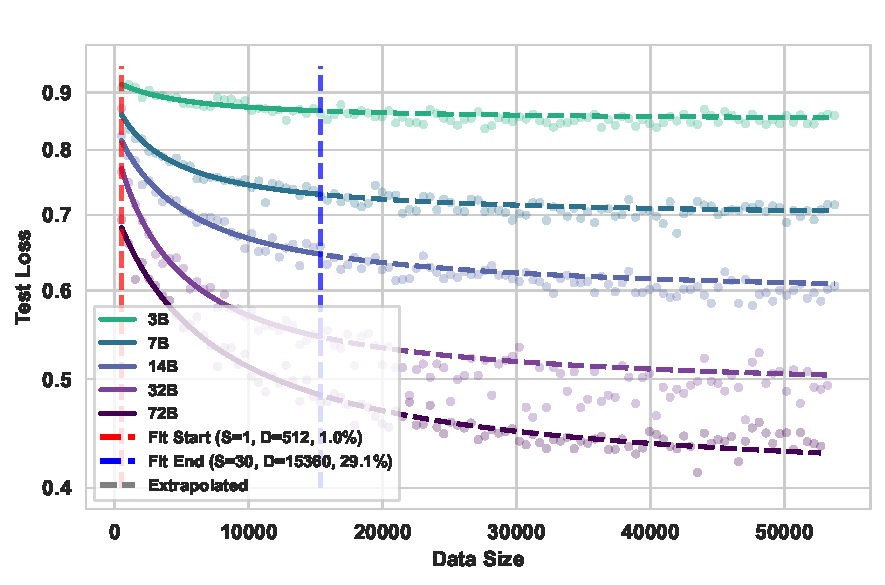
\includegraphics[width=\linewidth]{figures/fit_xh/fit_v3_inter_base_holdout_N_E_ErrRate.pdf}
        \caption{Intra-model prediction using the early 30\% of training steps.}
        \label{fig:v3_pred_a}
    \end{subfigure}
    \hfill
    \begin{subfigure}{0.48\textwidth}
        \centering
        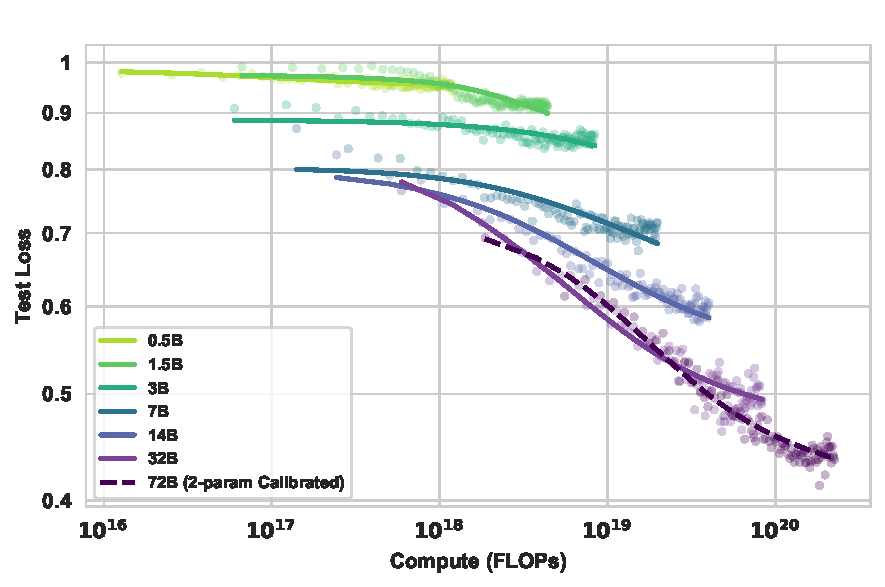
\includegraphics[width=\linewidth]{figures/fit_xh/fit_v3_intra_base_holdout_N_C_raw_ErrRate.pdf}
        \caption{Inter-model extrapolation for 72B under fixed shared shape.}
        \label{fig:v3_pred_b}
    \end{subfigure}
    \caption{Extrapolation of the loss decomposition model (Equation~\eqref{eq:v3_o2k}). 
    (a) Intra-model prediction using partial learning-curve observations. 
    (b) Inter-model extrapolation for 72B with global exponents fixed from smaller models.}
    \label{fig:v3_pred}
\end{figure}

We evaluate the extrapolation behavior of the loss–decomposition model (Equation~\eqref{eq:v3_o2k}) by applying it to the same experimental learning-curve data used in the main analysis, and by testing its performance under two complementary settings (Figure~\ref{fig:v3_pred}).

\paragraph{Intra-model prediction.}
Using only the first 30\% of training steps for each model, the fitted curves closely match the held-out portions(Figure~\ref{fig:v3_pred}a). This indicates that the internal S-shaped structure of the model provides a sufficiently strong inductive bias for completing a single learning curve from early observations. See Table~\ref{tab:fit_v3_intra} for detailed fitting result.

\paragraph{Inter-model extrapolation.}
We fit all global exponents and the model-limited term using models up to 32B, and then extrapolate the resulting shared functional form to 72B by calibrating only two model-specific parameters, $\lambda(72\text{B})$ and $D_0(72\text{B})$.
The extrapolated curve aligns well with the observed 72B trajectory across the full data range, reflecting that the functional shape inferred from smaller models remains compatible with larger-scale behavior under this light calibration.

The fit is reasonably strong, indicating that the proposed formulation may capture key structural tendencies of the underlying scaling behavior.


\begin{table}[H]
\centering
\caption{Fitting details for $L(N,D)$ using only 30\% of the training steps for each model.}
\label{tab:fit_v3_intra}
\begin{tabular}{lccc}
\toprule
\multirow{2}{*}{\textbf{Model Size}} & \multicolumn{3}{c}{\textbf{Base}} \\
\cmidrule(lr){2-4}
 & $D_0$ & $lambda$ & $R^2$ \\
\midrule
3B & 5109.6316 & 0.0734 & 0.995 \\
7B & 3725.6374 & 0.1882 & 0.995 \\
14B & 4554.7619 & 0.2520 & 0.995 \\
32B & 3576.0323 & 0.3279 & 0.995 \\
72B & 5861.6228 & 0.3084 & 0.995 \\
\bottomrule
\end{tabular}
\end{table}


% \begin{figure}
%     \centering
%     \includegraphics[width=\textwidth]{figures/fit_xh/fit_param_base_xh_N_E_D0_lambda_compare_source.pdf}
%     \caption{Fitted parameters}
%     \label{fig:placeholder}
% \end{figure}


\subsection{Discussion: Effective log--log slope}

To relate the loss decomposition model to the slope-based formulation used in the main text, we examine the local behavior of $L(N,D)$ in log--log coordinates with respect to the data scale $D$.  
Specifically, we define the effective slope
\[
k(N,D)\;:=\; -\,\frac{\partial \log L(N,D)}{\partial \log D},
\]
which corresponds to the exponent in a local power-law approximation of the form
$\log L \approx -k \log D + \text{const}$.

For the loss decomposition model (Equation~\eqref{eq:v3_o2k}), the induced $k(N,D)$ is a smooth function of $D$ that vanishes in both the low-data and high-data limits, and attains its maximum around the characteristic scale $D \approx D_0(N)$.  
Evaluating the slope at this point yields a natural definition of the maximal effective slope,

\begin{align}
\label{eq:v3_kn}
    k_{\max}(N)
    =
    \frac{K_{\max}}{1 + S(N)}, \\
    K_{\max}:= \frac{\beta}{2},\\
    S(N):=
    \frac{2\!\left(L_{\infty} + (N_0/N)^{\alpha}\right)}{\lambda(N)}.
\end{align}


The resulting $k_{\max}(N)$ depends only on the model size $N$ through the parameters of the loss decomposition, and is uniformly bounded by $K_{\max}=\beta/2$.

From this perspective, the slope function $k(N)$ adopted in the main analysis (Equation~\eqref{eq:efficiency_intro}) can be interpreted as a parsimonious, low-parameter approximation to the effective maximal slope $k_{\max}(N)$ in Eq.~\ref{eq:v3_kn}.
This establishes structural consistency between the two descriptions: the loss decomposition model potentially captures the finer-grained $(N,D)$-dependent behavior, while the main-text formulation summarizes its dominant $N$-dependent trend in a compact form.

\subsection{Conclusion}

The loss decomposition model captures key empirical characteristics of RL post-training scaling behavior.

However, several components remain underdetermined, including the construction of the learnable capacity $\lambda(N)$, the dependence of the characteristic dataset scale $D_0(N)$ on model size, the role of the pretraining process, and the impact of mismatches between pretraining and post-training task settings.

For these reasons, we present this model as an appendix-level discussion rather than a core component of the main text.
We encourage future work to build on this formulation to further investigate and refine scaling laws for LLM-based reinforcement learning.
